\documentclass[nooutcomes]{ximera}
%% handout
%% space
%% newpage
%% numbers
%% nooutcomes

%I added the commands here so that I would't have to keep looking them up
%\newcommand{\RR}{\mathbb R}
%\renewcommand{\d}{\,d}
%\newcommand{\dd}[2][]{\frac{d #1}{d #2}}
%\renewcommand{\l}{\ell}
%\newcommand{\ddx}{\frac{d}{dx}}
%\everymath{\displaystyle}
%\newcommand{\dfn}{\textbf}
%\newcommand{\eval}[1]{\bigg[ #1 \bigg]}

%\begin{image}
%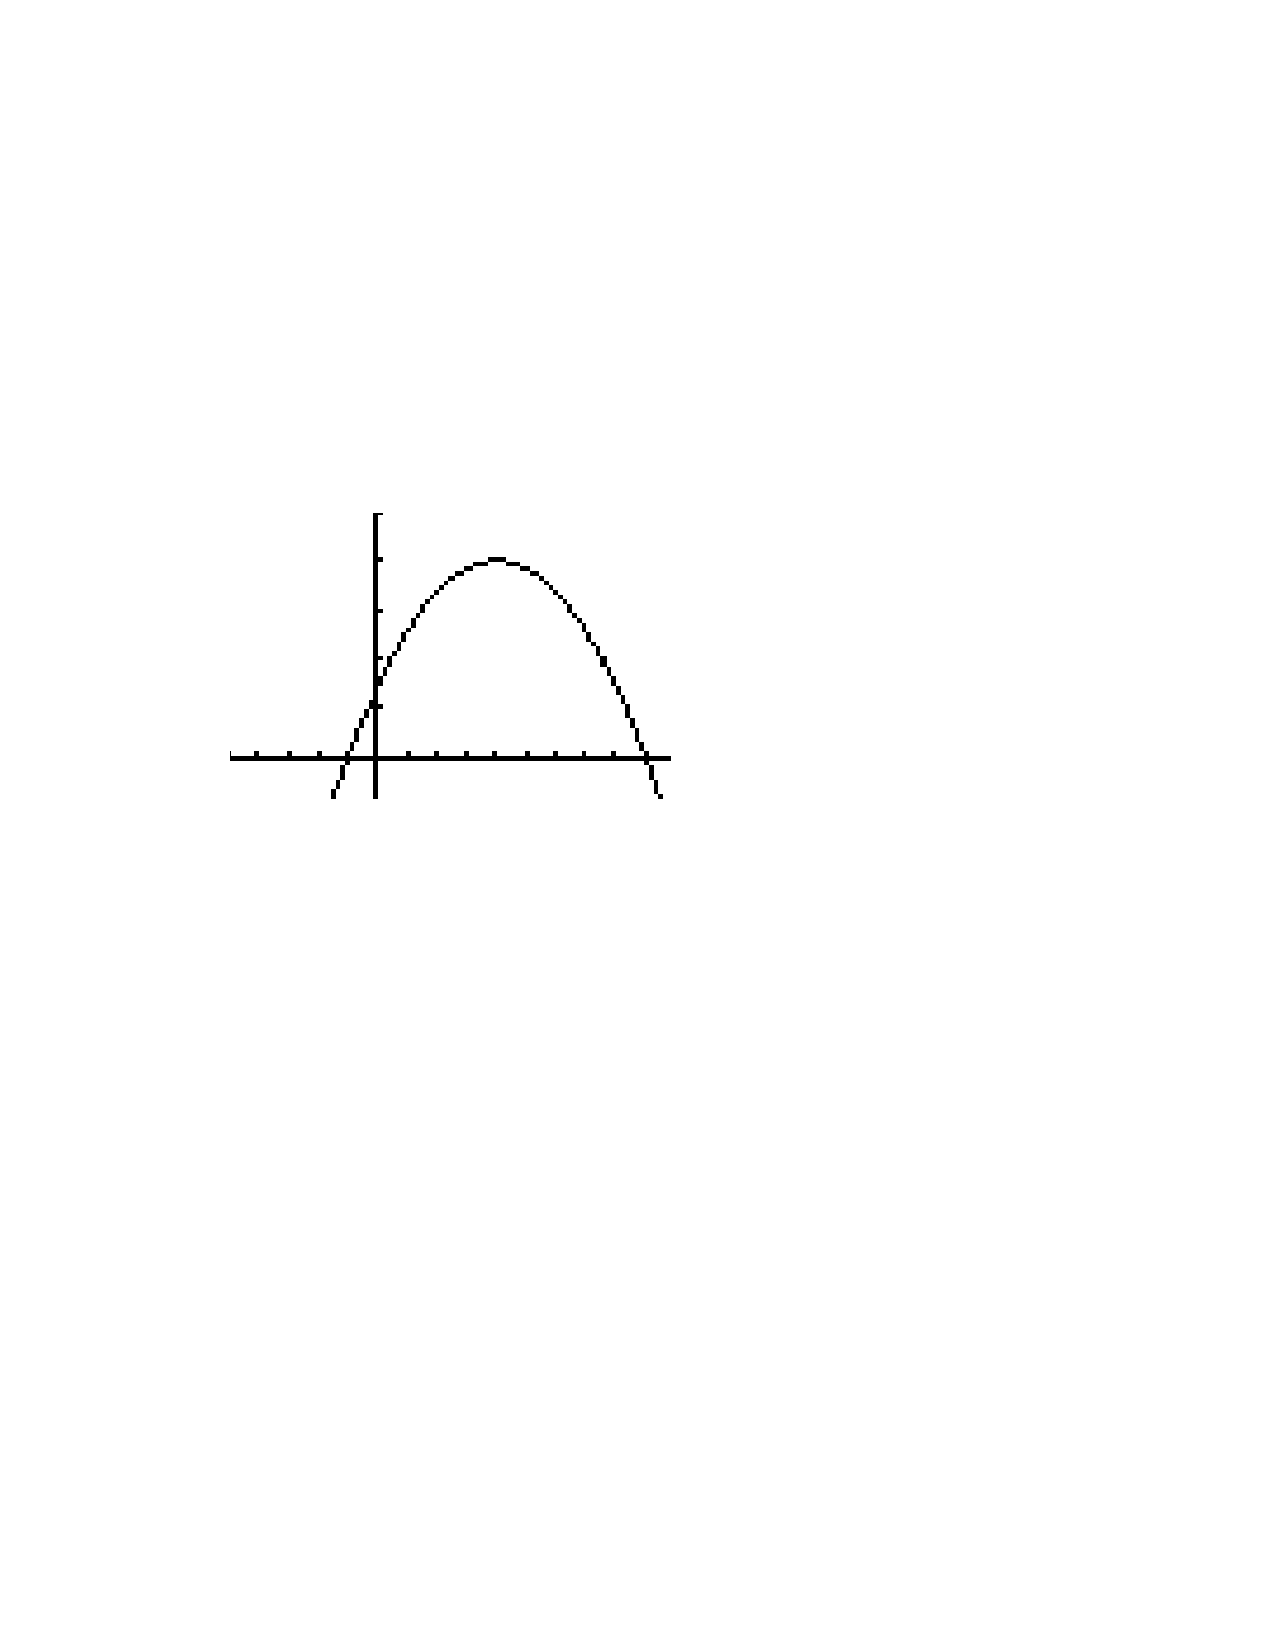
\includegraphics[trim= 170 420 250 180]{Figure1.pdf}
%\end{image}


\newcommand{\RR}{\mathbb R}
\renewcommand{\d}{\,d}
\newcommand{\dd}[2][]{\frac{d #1}{d #2}}
\renewcommand{\l}{\ell}
\newcommand{\ddx}{\frac{d}{dx}}
\newcommand{\dfn}{\textbf}
\newcommand{\eval}[1]{\bigg[ #1 \bigg]}

\usepackage{multicol}

\renewenvironment{freeResponse}{
\ifhandout\setbox0\vbox\bgroup\else
\begin{trivlist}\item[\hskip \labelsep\bfseries Solution:\hspace{2ex}]
\fi}
{\ifhandout\egroup\else
\end{trivlist}
\fi} %% we can turn off input when making a master document

\title{Recitation \#20 - 4.6 Mean Value Theorem (Solutions)}  

\begin{document}
\begin{abstract}		\end{abstract}
\maketitle

\section*{Warm up:} 
Heidi drives from her house in Columbus, OH to Tampa, FL for vacation.  Google maps says her driving distance is $1000$ miles.  The drive takes her $13$ hours.  The police send her a speeding ticket in the mail, saying she must have sped to arrive so quickly.  She is fighting the ticket, saying she just never stopped through the whole drive.  Can you prove she broke the $75$ mph speed limit at some point during her drive? 
		\begin{freeResponse}
		Let us define $s(t)$ to be the position function of Heidi after $t$ hours.  $s(t)$ will be continuous and differentiable because the location of a car is continuous and differentiable.  Heidi’s average speed for the whole trip is $\frac{1000}{13}\approx 76.9$ mph.  By the Mean Value Theorem, Heidi’s instantaneous speed was $76.9$ mph at some point of her trip: hence, she broke the $75$ mph speed limit.  
		\end{freeResponse}	
		
		
		

	
	
	
	
	

\section*{Group work:}



%problem 1
\begin{problem}
Does the function given in the graph below satisfy the hypotheses of the Mean Value Theorem in the interval $[-1,6]$?  If so, estimate the values of all numbers $c$ that satisfy the conclusion of the Mean Value Theorem.  
	\begin{image}
	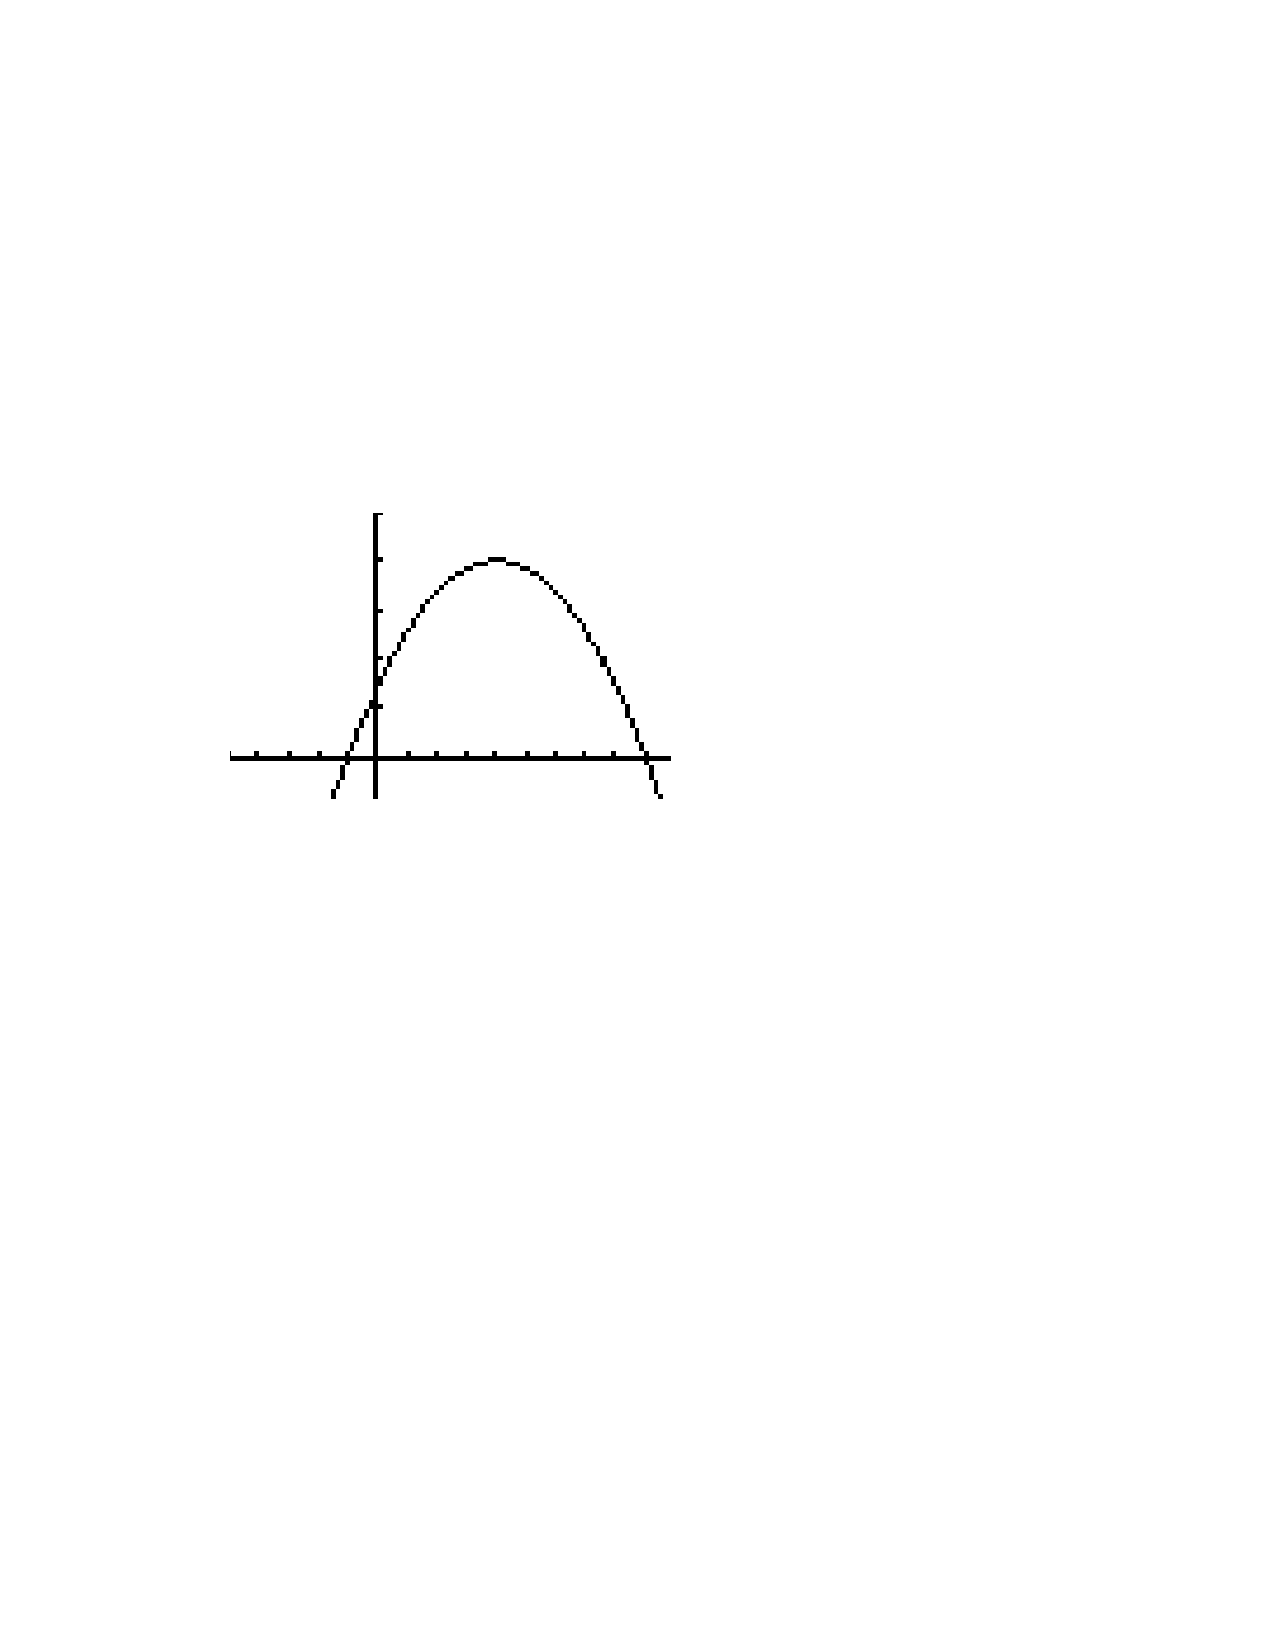
\includegraphics[trim= 100 420 320 160]{Figure1.pdf}
	\end{image}
	
		\begin{freeResponse}
		The function is continuous on $[-1,6]$ and differentiable on $(-1,6)$: hence it satisfies the hypothesis of the Mean Value Theorem.
			\begin{image}
			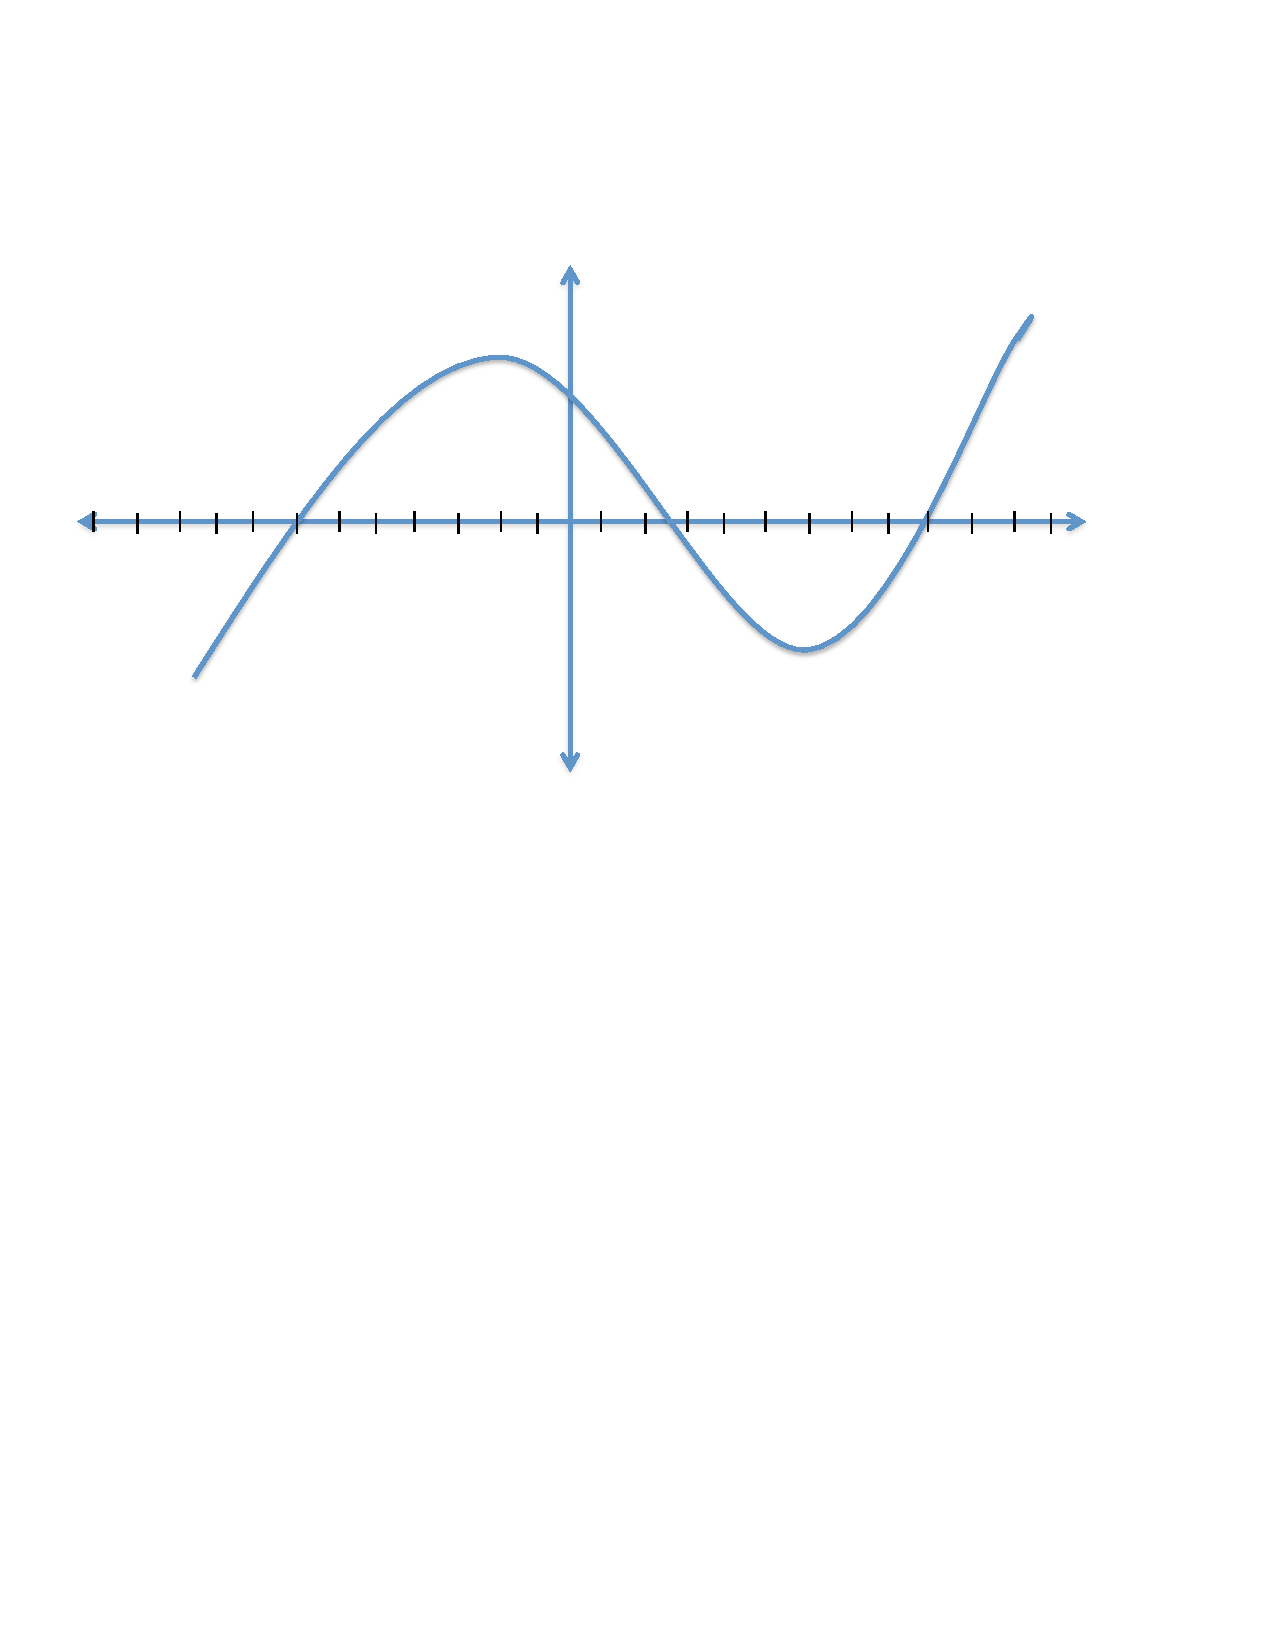
\includegraphics[trim= 100 460 320 190]{Figure2.pdf}
			\end{image}
			
		\end{freeResponse}
		
		
		

\end{problem}















%problem 2
\begin{problem}
Verify that the given function satisfies the hypotheses of the Mean Value Theorem in the given interval.  Then algebraically find all numbers $c$ that satisfy the conclusion of the Mean Value Theorem.  Using the graph provided, label the point(s) $c$ and sketch the secant line and the tangent line at $c$
$$ f(x) = \frac{x}{x+2} \qquad \text{on } [1,4] $$.
	\begin{image}
	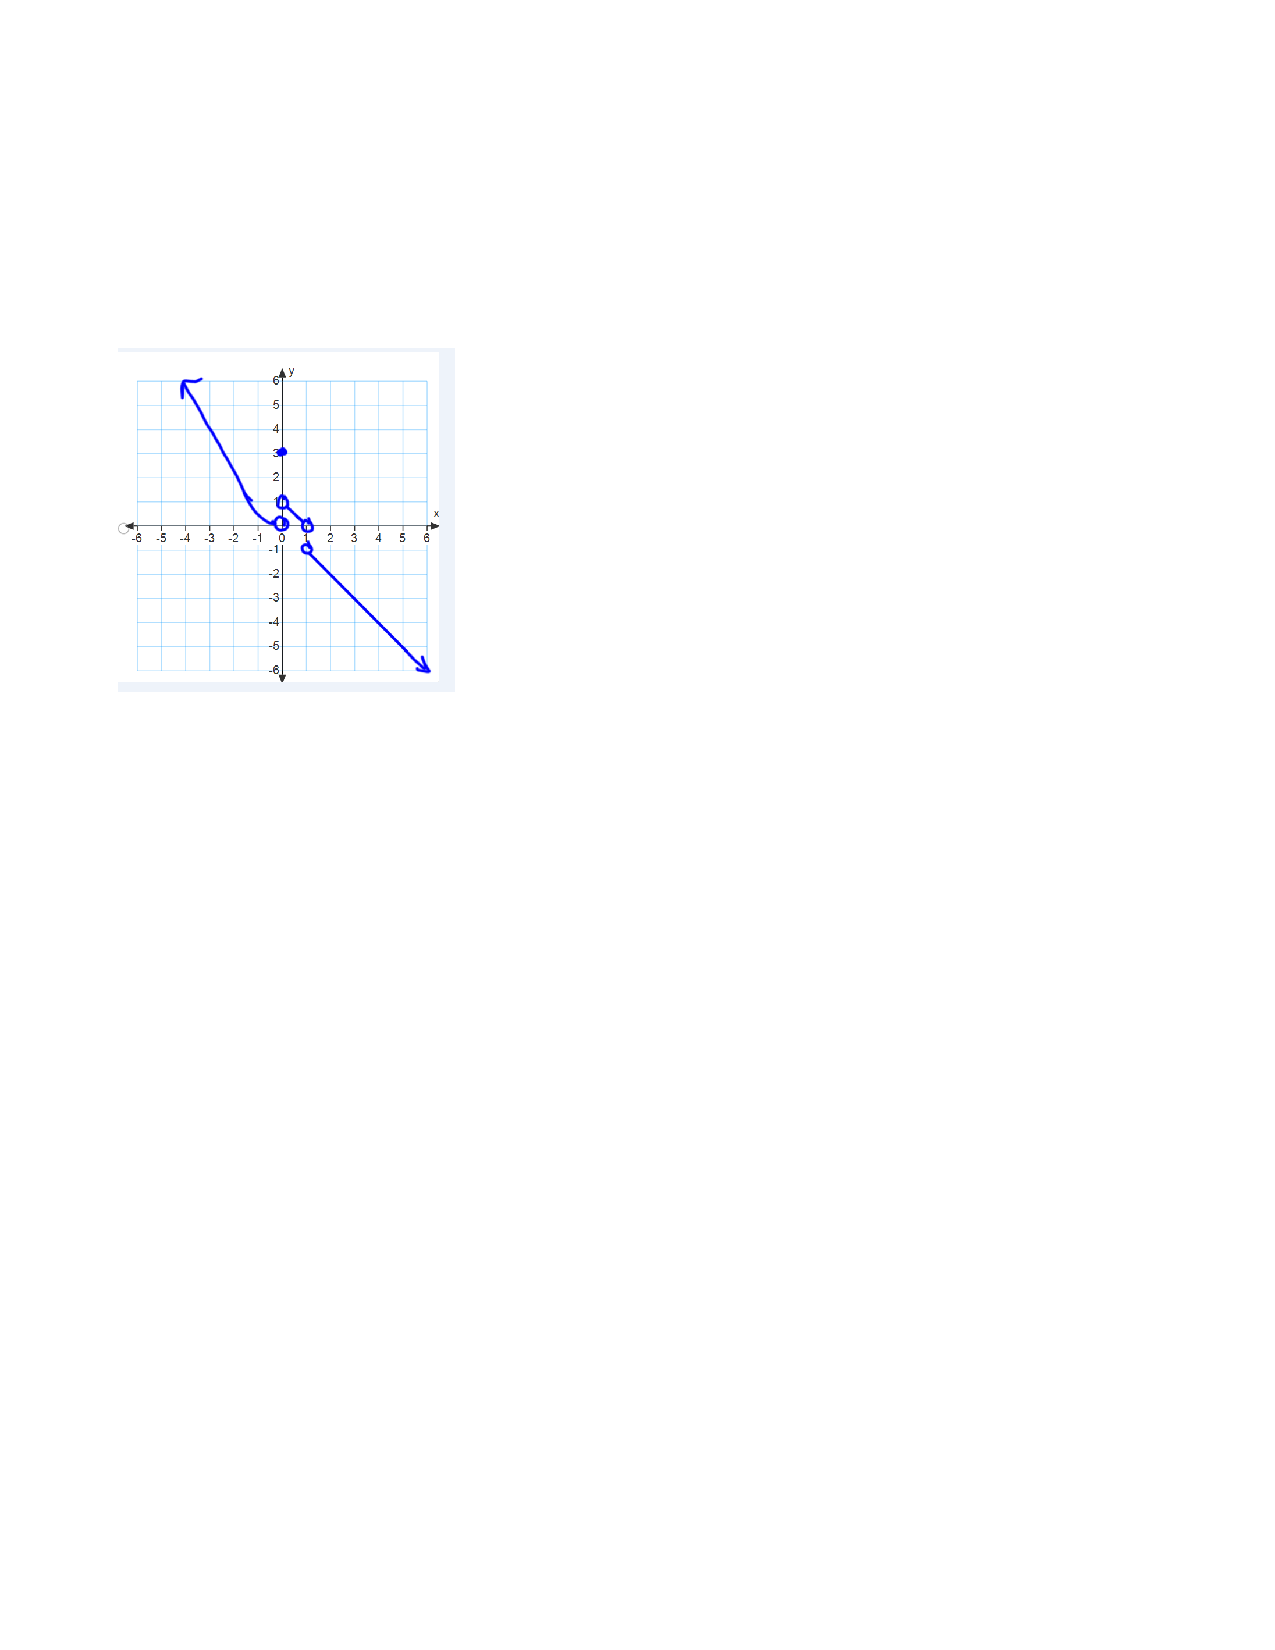
\includegraphics[trim= 120 480 350 180]{Figure3.pdf}
	\end{image}
		\begin{freeResponse}
		The function $f(x) = \frac{x}{x+2}$ is continuous on $[1,4]$ and differentiable on $(1,4)$ since it is a rational function, and is therefore continuous and differentiable on its domain.  Therefore, $f$ satisfies the hypotheses of the Mean Value Theorem.  We have that
		$$ f'(x) = \frac{(x+2)(1) - x(1)}{(x+2)^2} = \frac{2}{(x+2)^2} $$
		$$ \frac{f(4) - f(1)}{4-1} = \frac{\frac{2}{3} - \frac{1}{3}}{3} = \frac{1}{9} $$
		So we are looking to find all points $c \in (1,4)$ which satisfy that $ f'(c) = \frac{1}{9} $.  So we solve:
		$$ \frac{2}{(c+2)^2} = \frac{1}{9} $$
		$$ (c+2)^2 = 18 $$
		$$ c = \sqrt{18} - 2 = 3\sqrt{2} - 2 $$
		Note that we omitted $-\sqrt{18} - 2$ above because it is not in the interval $(1,4)$.  Therefore, $c = 3\sqrt{2} - 2$.
		
		\begin{image}
		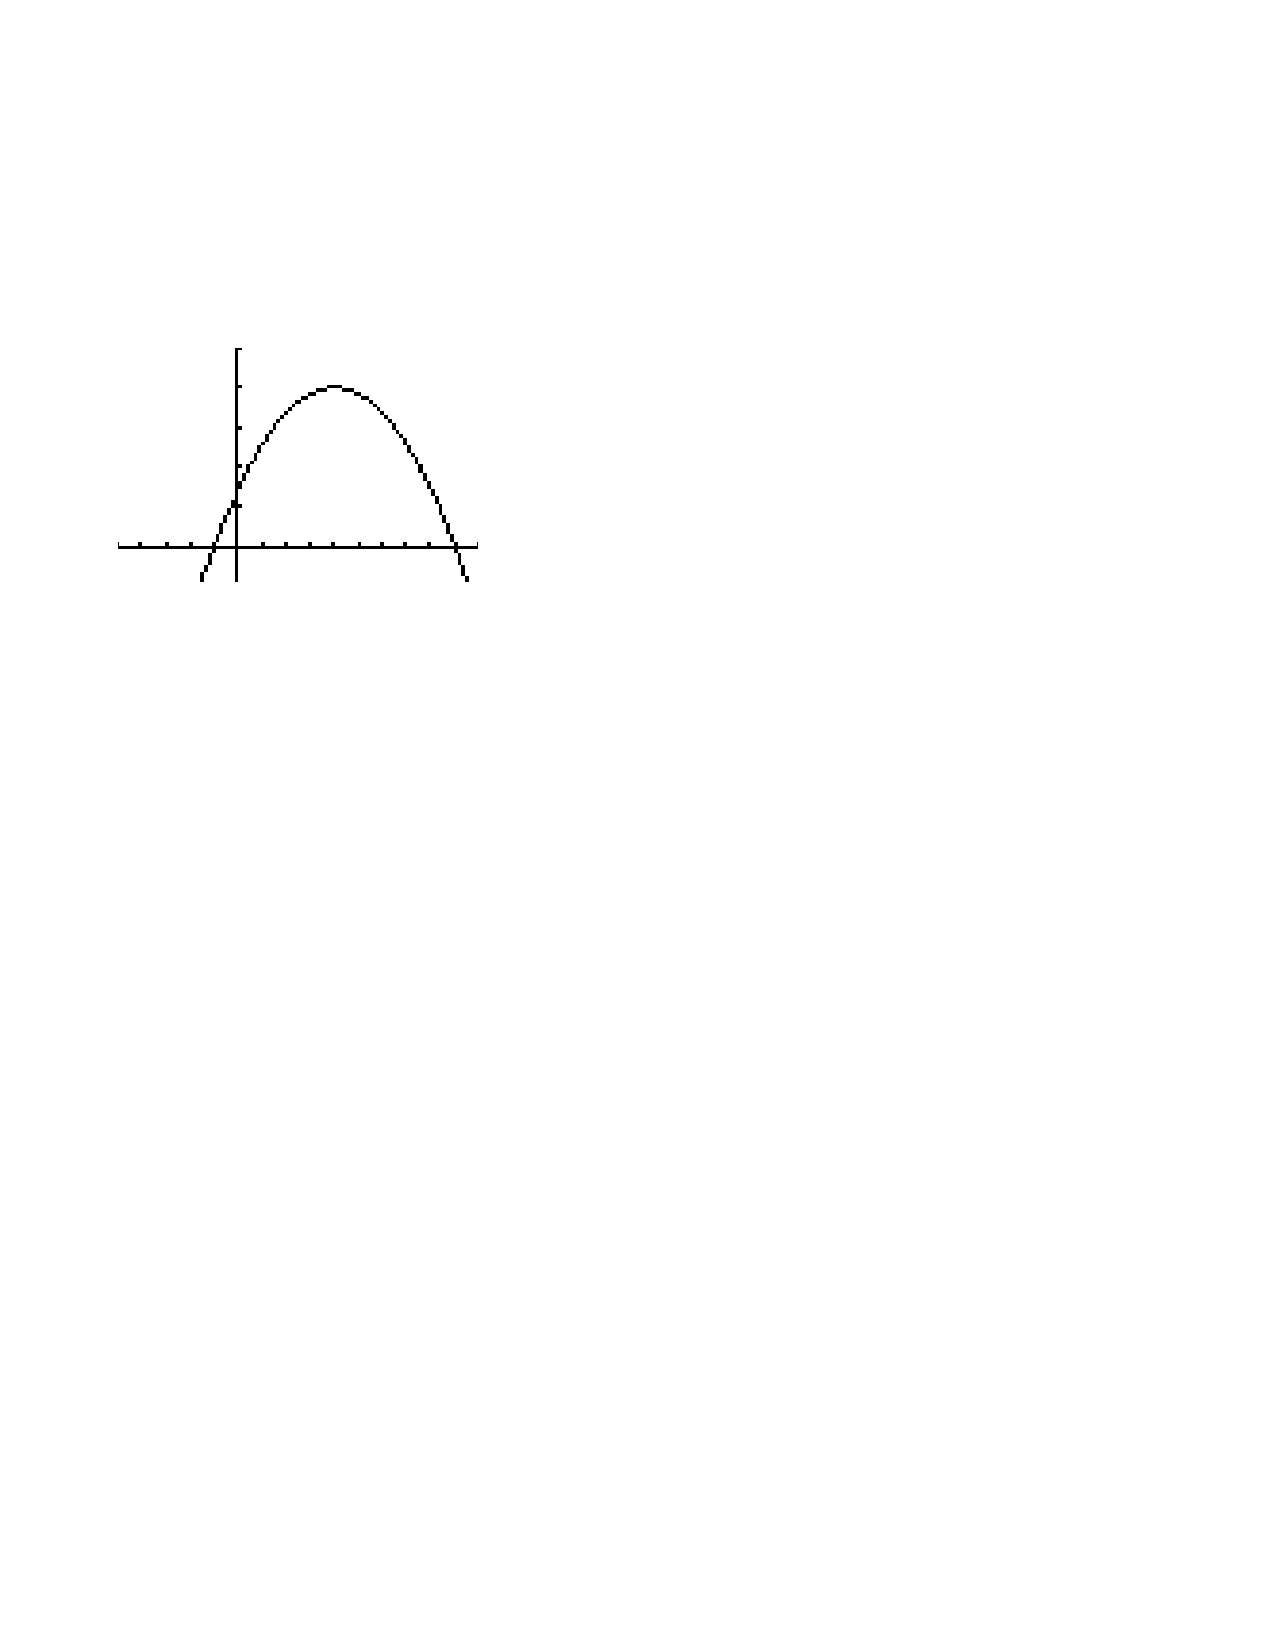
\includegraphics[trim= 130 420 250 180]{Figure4.pdf}
		\end{image}
		
		\end{freeResponse}
		
		
\end{problem}









	
	
	
	
	
	
	
	
			
			

%problem 3
\begin{problem}
Let $f(x) = (x-3)^{-2}$.  Show that there is no value $c$ in $(1,4)$ such that $f(4) - f(1) = f^{\prime}(c) (4-1)$.  Why does this not contradict the Mean Value Theorem?
		\begin{freeResponse}
		First notice that 
		$$f(4)-f(1) = 1^{-2} - (-2)^{-2} = 1-\frac{1}{4} = \frac{3}{4}$$
		and so we are looking for a value $c$ such that 
		$$3 f^\prime (c) = \frac{3}{4} \quad \Longrightarrow \quad f^\prime (c) = \frac{1}{4} $$
		Then since $f'(x) = \frac{-2}{(x-3)^3}$, we can compute:
		$$ f'(c) = \frac{-2}{(c-3)^3} := \frac{1}{4}$$
		$$ (c-3)^3 = - 8 $$
		$$ c = 3 - 2 = 1 $$
		But $1$ is not in the interval $(1,4)$.  This does not contradict the Mean Value Theorem since $f$ is not continuous at $x=3$.
		
		\begin{image}
		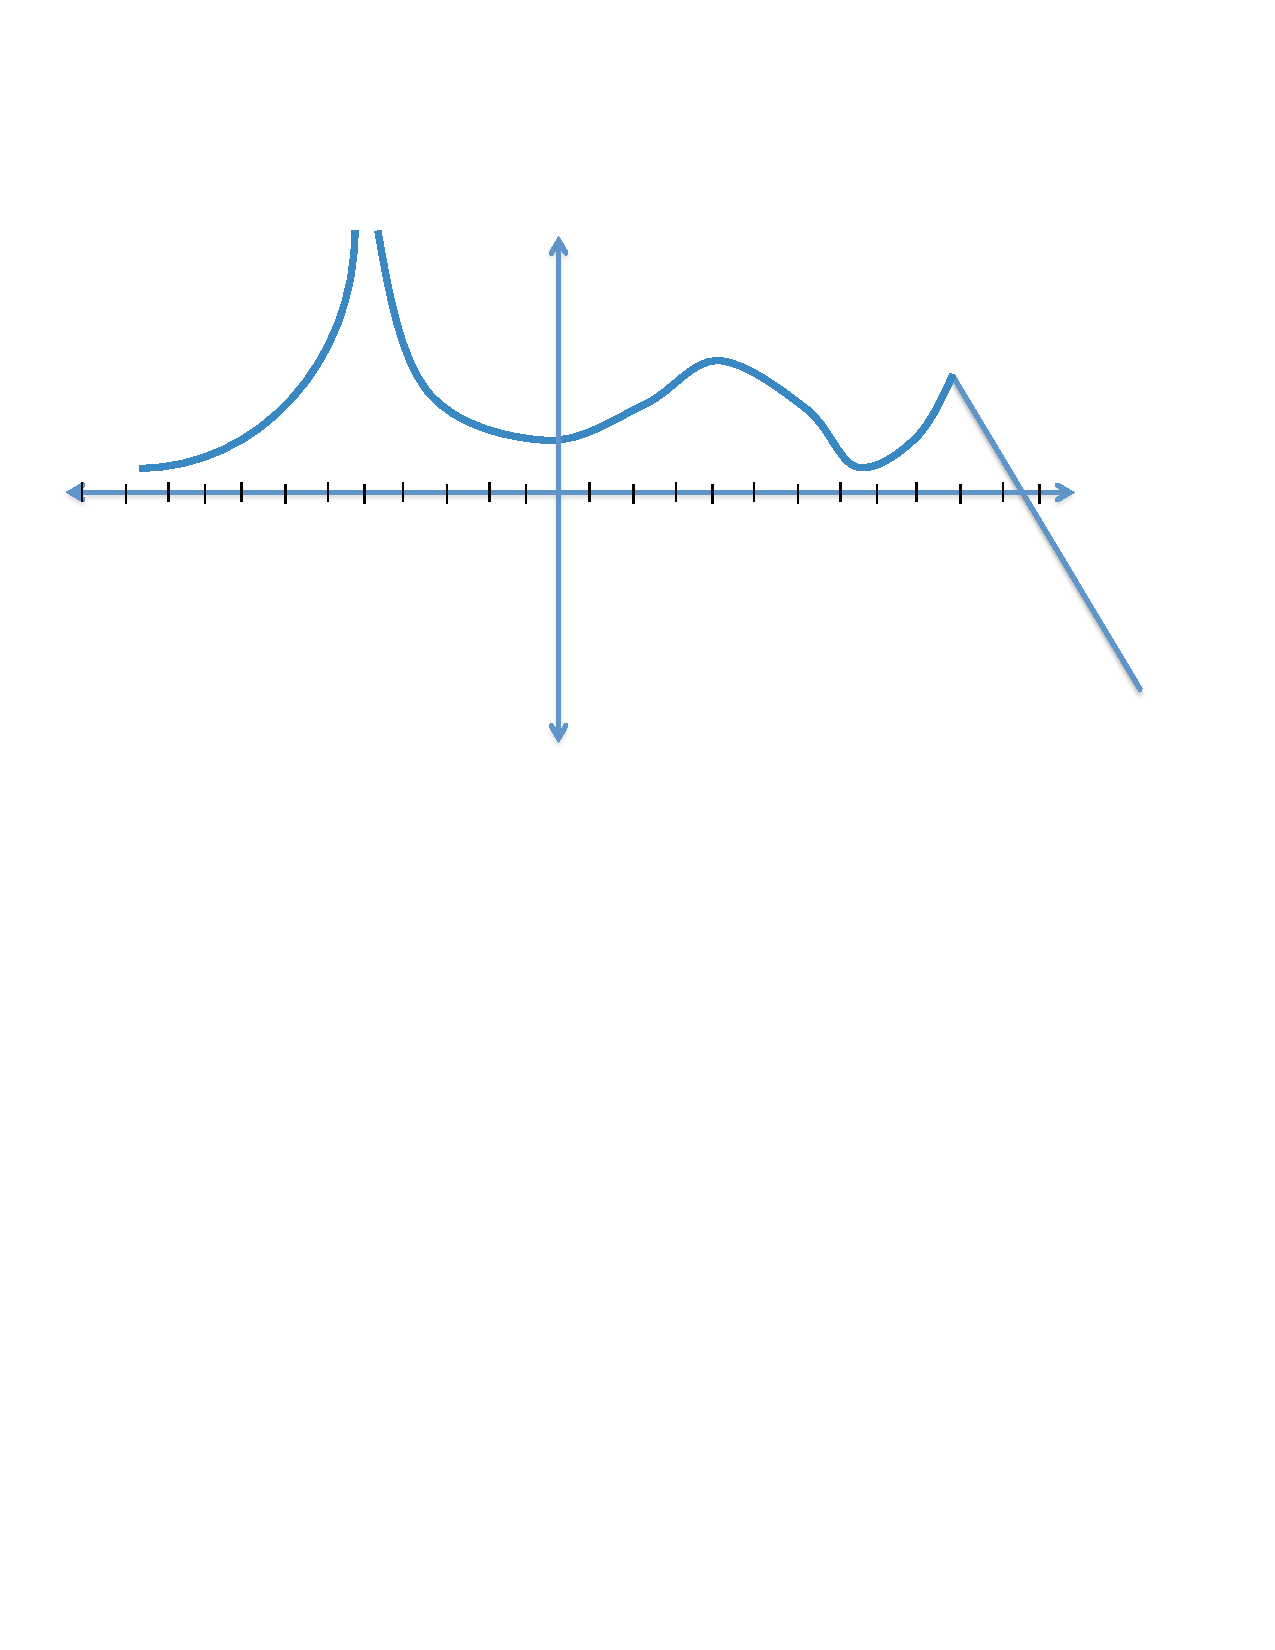
\includegraphics[trim= 100 440 300 210]{Figure5.pdf}
		\end{image}
		
		\end{freeResponse}
			
			
		
\end{problem}















%problem 4
\begin{problem}
Two runners start a race at the same time and finish in a tie.  Prove that at some time during the race they have the same speed.  (Hint:  Consider the function $h(t)=f(t)-g(t)$, where $f(t)$ and $g(t)$ are the position of the first and second runner at time $t$, respectively.)
		\begin{freeResponse}
		Let $f(t)$ be the position of the first runner at time $t$, and let $g(t)$ be the position of the second runner at time $t$.  Let $T$ denote the time that the two runners finish the race (which is the same, since they finish in a tie).  Also, let $h(t) = f(t) - g(t)$.  Since $h(0) = 0$ and $h(T) = 0$, by Rolle's Theorem there exists some $c$ with $0 < c < T$ such that $h'(c)=0$.  But since $h^\prime (t) = f^\prime (t) - g^\prime (t)$, we have that $f^\prime (c) = g^\prime (c)$.  Therefore, the runners hae the same speed at time $c$.  
		
		\begin{image}
		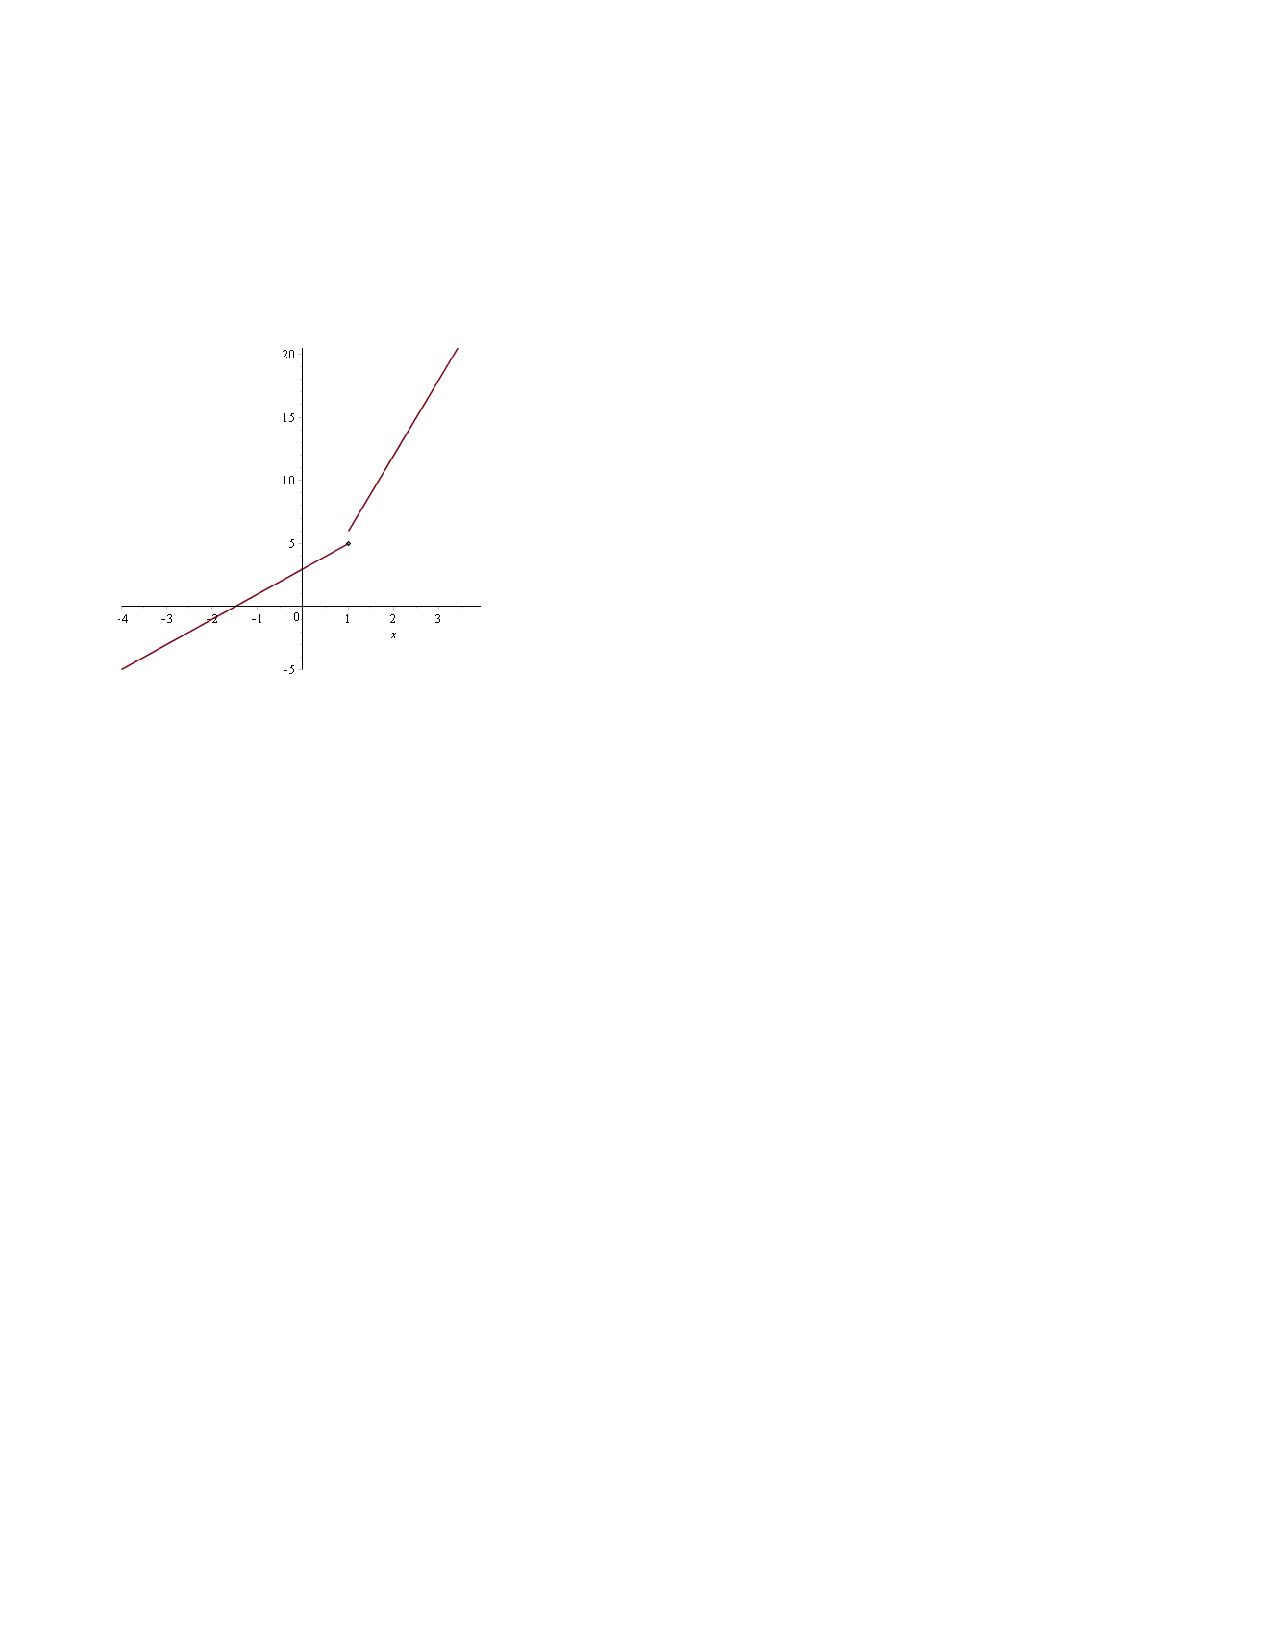
\includegraphics[trim= 100 440 300 180]{Figure6.pdf}
		\end{image}
		
		\end{freeResponse}
			
			
	
\end{problem}






	
	
	
	
	
	
	
	
	

	










								
				
				
	














\end{document} 


















